\documentclass[mirror, portugues]{revdetua}
%
% Valid options are:
%   portugues --------- main language is Portuguese
%   final ------------- final version (default)
%   times ------------- use times (postscript) fonts for text
%   mirror ------------ prints a mirror image of the paper (with dvips)
%   visiblelabels ----- \SL, \SN, \SP, \EL, \EN, etc. defined
%   invisiblelabels --- \SL, \SN, \SP, \EL, \EN, etc. not defined (default)
%
% Note: the final version should use the times fonts
% Note: the really final version should also use the mirror option
%

\usepackage[portuguese]{babel}
\usepackage[utf8]{inputenc}
\usepackage{amsmath} 
\usepackage{comment}
\usepackage{algorithm}
\usepackage{algpseudocode}
\floatname{algorithm}{Algoritmo}
\usepackage{graphicx}
\usepackage[justification=centering]{caption}
\usepackage{float}
%-------------------------------------
% compiling:
% Recipe: xelatex
% Recipe: pdflatex -> bibtex -> pdflatex -> pdflatex
% Recipe: xelatex
%
% notas:
% rever se algorimtos e imagens estão onde devem
%-------------------------------------
\begin{document}

\Header{02}{3}{Dezembro}{2024}{1}

\title{Maximum Weight Cut Problem}
% MUDAR TITULO ALLEZ ALLEZ ALGO COM RANDOMIZADO
\author{Hugo Veríssimo - 124348 - hugoverissimo@ua.pt}
\maketitle

\begin{abstract}
... abstrato em ingles
\end{abstract}

\begin{resumo}
Este relatório apresenta a implementação e comparação de dois métodos para resolver o problema \textit{Maximum Weight Cut}: uma pesquisa exaustiva e uma heurística gulosa. O problema \textit{Maximum Weight Cut} con ESTE É O ANTIGO FAZER NOVO
\end{resumo}

\section{Introdução}

ja se analisou no outro relatorio a descrição do problema \textit{Maximum Weight Cut}, e ns q, super fixe

este relatoria visa explorar algoritmos com um certo grau de estocacidade/aletorieda com vista em otimizar a complexidade e as solucoes.

para alem disso os resultados são comparados aos obtidos anteriormente

serao entao implexmentados 3 algoritmos, nomeadamente: ... e ...

\section{Metodologia da Análise}

vamos usar o python por ter o modulo random e outros

ns q vamos usar os ficheiro tal e tal 

e para testar os algortimos serão testados os graficos do Gset e criados por nós com o ficheiro tal

Graphs for the Computational Experiments: mine and elearnig ou links and gset

\section{Algoritmo de 1}

este algoritmo é o tipico "aleatorio" que consite na geracao de solucoes aleatorias, e a comparacao das mesmas, e a escolha da melhor solucao, nao havendo qualquer componente deterministica (?)

para garantir que n ha solucoes testadas mais q uma vez, as solucoes ja testadas sao guardadas num set, e antes de testar uma nova solucao, verifica se esta ja foi testada, e se sim, passa para a proxima solucao evitando o calculo do peso do corte, uma operacao que é cara

este algortimo ou quando atingir o numero de solucoes a gerar ou quando todas as solucoes possiveis foram testadas, ou seja, quando o numero de solucoes testadas for igual a $2^n$

\begin{algorithm}[H]
\raggedright
\textbf{Entrada:}

- lista de arestas e respetivos pesos (\textit{edges})

- número de vértices (\textit{n\_nodes})

- número de soluções a gerar (\textit{solutions})\\
\textbf{Saída:} subconjuntos \textit{S} e \textit{T}, peso do corte (\textit{weight}) \\
\hrule 
\caption{NOME DO ALGORTIMO}
\begin{algorithmic}[1]
    \State \texttt{best\_solution} $\gets$ \texttt{None}
    \State \texttt{weight} $\gets$ 0
    \State \texttt{seen\_solutions} $\gets$ empty set
    \For{$i \gets 1$ \textbf{to} \texttt{solutions}}
        \State \texttt{partition} $\gets$ random partition of the nodes
        \If {\texttt{length}(\texttt{seen\_solutions}) $=$ $2^{\texttt{n\_nodes}}$}
            \State \textbf{break}
        \EndIf
        \State \texttt{partition\_hash} $\gets$ hash the partition
        \If {\texttt{partition\_hash} $\in$ \texttt{seen\_solutions}}
            \State \textbf{continue}
        \EndIf
        \State Add \texttt{partition\_hash} to \texttt{seen\_solutions}
        \State \texttt{new\_cut\_weight} $\gets$ compute the cut weight
        \If {\texttt{new\_cut\_weight} $>$ \texttt{weight}}
            \State \texttt{weight} $\gets$ \texttt{new\_cut\_weight}
            \State \texttt{best\_solution} $\gets$ copy of \texttt{partition}
        \EndIf
    \EndFor
    \State \texttt{S} $\gets$ set of nodes assigned to $0$ in \texttt{best\_solution}
    \State \texttt{T} $\gets$ set of nodes assigned to $1$ in \texttt{best\_solution}
    \Return \texttt{S}, \texttt{T}, \texttt{weight}
\end{algorithmic}
\end{algorithm}
    
quando a complexidade, este algortimo, a parte mais cara é o loop que corre no maximo \texttt{solutions} vezes, e dentro dele, a complexidade é O(n + m) por gerar uma particao aleatoria e calcular o peso do corte, logo a complexidade final é $O((m + m) \times \texttt{solutions})$, tendendo para $O(n^2)$ para grafos densos e um n grande




\section{Algoritmo de 2}

%https://apps.dtic.mil/sti/citations/ADA185547

o segundo algortimo a ser implementado é o Simulated Annealing, que é um algoritmo de otimizacao global, que procura a melhor solucao possivel, e que é baseado no processo de arrefecimento de metais, que consiste em arrefecer um metal a uma taxa controlada, para que os atomos se organizem de forma a minimizar a energia do sistema. ns q, o algortimo simulated Annealing consite em ... e é heuristico e ns q e random (referencias)

este algortimo já foi implementado no problema max cut por exemplo \cite{SAT15}

neste caso tem como componente aleatorio a selecao de uma solucao inicial e a aceitacao de solucoes piores, com uma probabilidade que decresce com o tempo, mas sendo esta aceite smp que a solucao for melhor que a anterior (determinisico)

\begin{figure}[h]
    \centering
    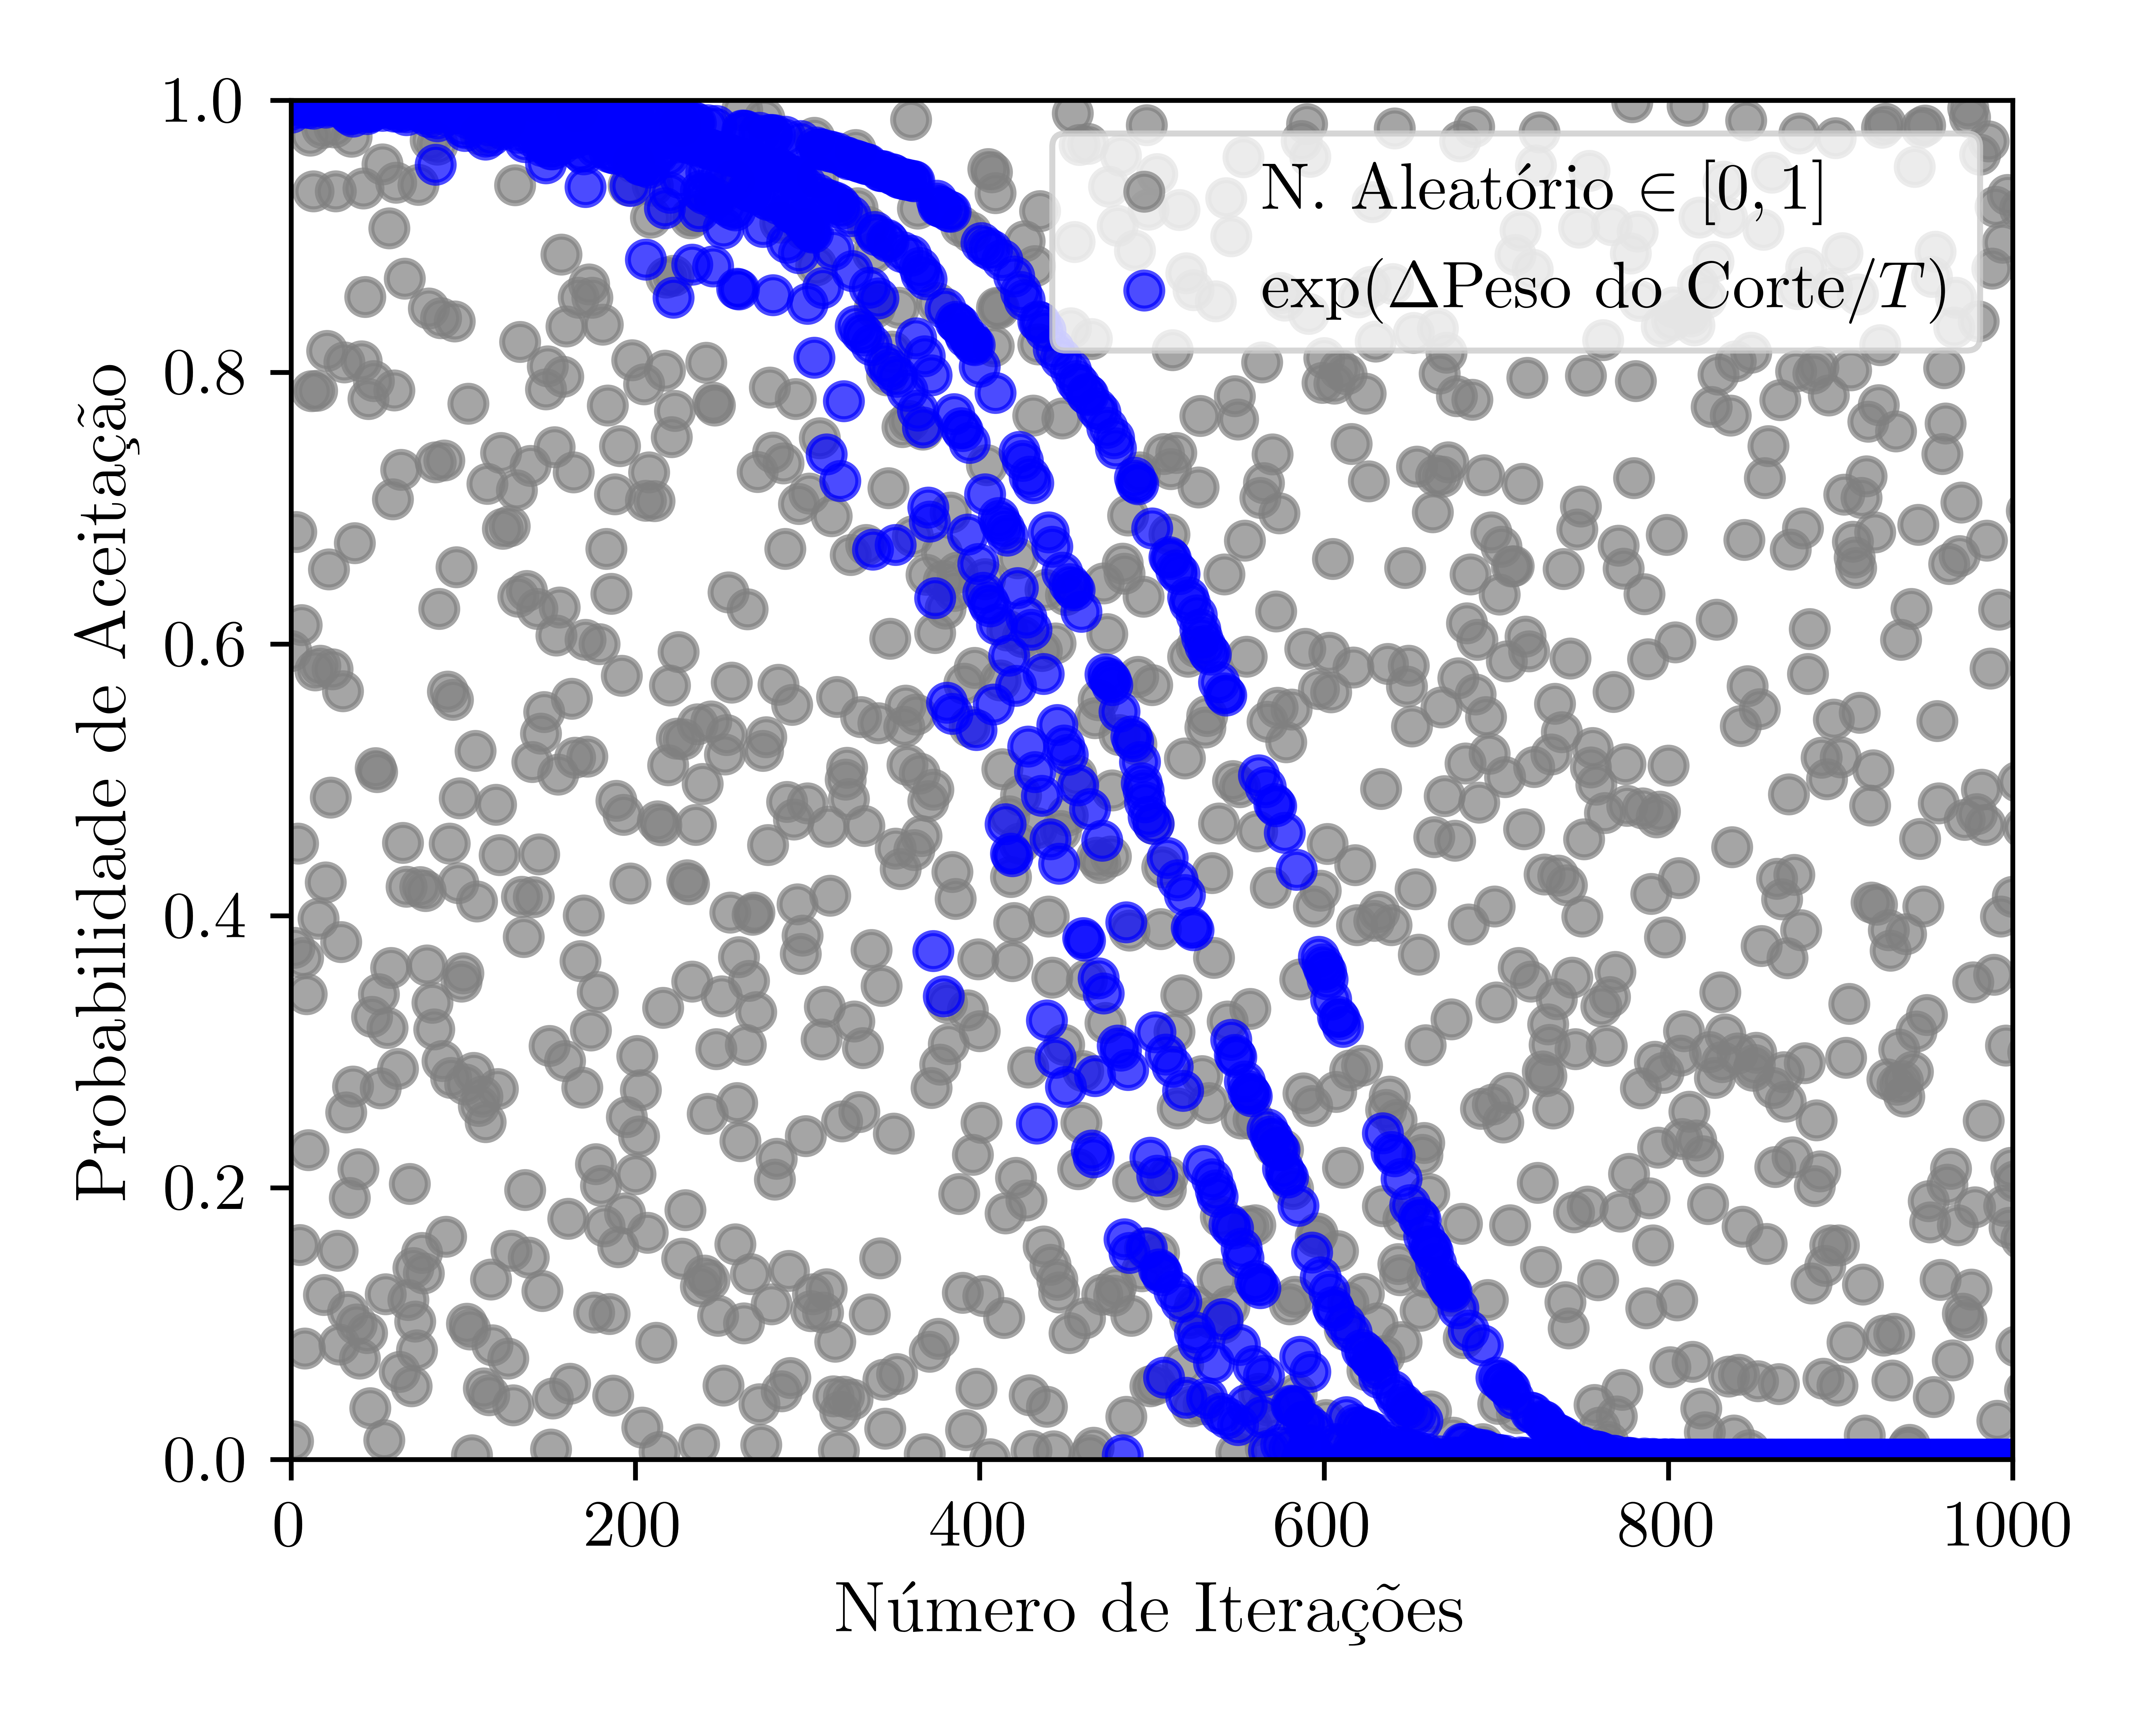
\includegraphics[width=0.45\textwidth]{../assets/SA_DecrAceit.png}
    \caption{ver que a aceitacao diminui com as iteracaoes por causa do arreficmento e bla bla, G59 usado e seed do SA 124348}
    \label{fig:sa_aceitacao}
\end{figure}

por ser sensivel a solucao inicial, é interessante testar diferentes solucoes iniciais, e por isso o algoritmo deve ser corrido um numero de vezes

neste algoritmo não ha garantia de que cada sol so é testada uma vez, por opção propria. visto que a probabilidade de testar a mesma solucao é dada por:

\dots

para grafos de maiores dimensões, esta prob torna-se muito baixa, e por isso a probabilidade de testar a mesma solucao é baixa, fazendo com que o processo de comparar solucoes ja testadas possa prejudicar a eficiencia do algoritmo 

o algortimo para quando a temperatura é menor que $10^{-3}$, pelo que o numero de iteracoes é variavel e depende do valor da temperatura inicial e da taxa de arrefecimento

\begin{algorithm}[H]
\raggedright
\textbf{Entrada:}

- lista de arestas e respetivos pesos (\textit{edges})

- temperatura (\textit{Temp})

- taxa de arrefecimento (\textit{cooling\_rate})\\
\textbf{Saída:} subconjuntos \textit{S} e \textit{T}, peso do corte (\textit{best\_cut}) \\
\hrule 
\caption{\textit{Simulated Annealing}}
\begin{algorithmic}[1]
    \State \texttt{partition} $\gets$ random partition of the nodes
    \State \texttt{best\_partition} $\gets$ \texttt{partition}
    \State \texttt{current\_cut} $\gets$ compute the cut weight
    \State \texttt{best\_cut} $\gets$ \texttt{current\_cut}
    \While{\texttt{Temp} \ensuremath{>} \ensuremath{10^{-3}}}
        \State \texttt{node} $\gets$ randomly select a node
        \State Flip the partition of \texttt{node} in \texttt{partition}
        \State \texttt{new\_cut} $\gets$ compute the new cut weight
        \State \texttt{cost\_diff} $\gets$ \texttt{new\_cut} $-$ \texttt{current\_cut}
        \If{\texttt{cost\_diff} \ensuremath{>} 0 \textbf{or} random number $\in$ [0, 1] \ensuremath{<} $e^{\ensuremath{\texttt{cost\_diff} / \texttt{Temp}}}}$
            \Comment Accept the move
            \State \texttt{current\_cut} $\gets$ \texttt{new\_cut}
            \If{\texttt{new\_cut} \ensuremath{>} \texttt{best\_cut}}
                \State \texttt{best\_cut} $\gets$ \texttt{new\_cut}
                \State \texttt{best\_partition} $\gets$ \texttt{partition}
            \EndIf
        \Else
            \Comment Reject the move
            \State Revert the partition of \texttt{node} in \texttt{partition}
        \EndIf
        \State \texttt{Temp} $\gets$ \texttt{Temp} \ensuremath{\times} \texttt{cooling\_rate}
    \EndWhile
    \State \texttt{S} $\gets$ set of nodes assigned to $0$ in \texttt{best\_partition}
    \State \texttt{T} $\gets$ set of nodes assigned to $1$ in \texttt{best\_partition} \\
    \Return \texttt{S}, \texttt{T}, \texttt{best\_cut}
\end{algorithmic}
\end{algorithm}

- complexidade on4 ?

tendo em conta a complexidade do algortimo, o gerar uma particao inicial envolve o(n) pq vai vertice a evrtice atribuir determinado subt. depois o valvulo do current cut envolve o(m) visto q corre a lista de todos os vertices

depois corre o loop K vezes

esolhe um nó e muda a sua partição o(1), recalcula o novo peso do corte o(m) e depois compara o novo corte com o anterior o(1) e se for melhor atualiza o corte e a particao o(1)

ou seja a complexidade é O(m) * K

K é dado por:

\begin{align*}
    &T_0 \cdot (\text{cooling\_rate})^k \le 10^{-3} \\
    \Leftrightarrow\ &  k \geq  \frac{\log\left(\frac{10^{-3}}{T_0}\right)}{\log(\text{cooling\_rate})} \\
    \Leftrightarrow\ & k = \left\lceil \frac{\log\left(\frac{10^{-3}}{T_0}\right)}{\log(\text{cooling\_rate})} \right\rceil
\end{align*}

logo a complexidade final é dada por $O(m) \approx O(n^2)$ para grafos densos , pq k é uma constante que não depende nem de m nem de n 

%https://apps.dtic.mil/sti/citations/ADA185547 O(n4)



\section{Algoritmo de 3}

este algoritmo consiste numa heuristica gulosa, que consiste em iterar por todos os vertices e trocar a sua particao, verificando se a solucao é melhor, e se for, atualiza a solucao, e quanto iterar por todos e nao melhorar em nenhum para.

contudo isto tornava o algoritmo muito lento, apesar dos bons repertidos, para isso foi adicionado um fator de ajuste do maximo de iteracoes (\textit{itLim}), que é o numero de arestas vezes o fator de ajuste, evitando assim que o algoritmo corra indefinidamente

como o algoritmo é guloso, a solucao final depende da solucao inicial, gerada aleatoriamente, e por isso o algoritmo deve ser corrido varias vezes, para garantir uma maior probabilidade a melhor solucao é encontrada

neste algoritmo, como a unica componente aleatoria é a particao inciial e como todas as alteracoes sao feitas em diracao a melhor solucao, o algoritmo nunca ira testar a mesma solucao duas vezes, pelo que nao é necessario guardar as solucoes ja testadas

\begin{algorithm}[H]
\raggedright
\textbf{Entrada:}

- lista de arestas e respetivos pesos (\textit{edges})

- número de vértices (\textit{n\_nodes})

- fator de ajuste do máximo de iterações (\textit{itLim})\\
\textbf{Saída:} subconjuntos \textit{S} e \textit{T}, peso do corte (\textit{weight}) \\
\hrule 
\caption{NOME DO ALGORTIMO}
\begin{algorithmic}[1]
    \State \texttt{partition} $\gets$ random partition of the nodes
    \State \texttt{cut\_weight} $\gets$ compute the cut weight
    \State \texttt{improved} $\gets$ \texttt{True}
    \State \texttt{it\_limit} $\gets$ \texttt{len(edges)} \ensuremath{\times} \texttt{itLim}

    \While{\texttt{improved} \textbf{and} \texttt{it\_limit} \ensuremath{>} 0}
        \State \texttt{it\_limit} $\gets$ \texttt{it\_limit} $ - 1$
        \State \texttt{improved} $\gets$ \texttt{False}
        \For{\texttt{node} \textbf{in} \texttt{range}(\texttt{n\_nodes})}
            \State Flip the partition of \texttt{node} in \texttt{partition}
            \State \texttt{new\_cut\_weight} $\gets$ compute the cut weight
            \If{\texttt{new\_cut\_weight} \ensuremath{>} \texttt{cut\_weight}}
                \State \texttt{cut\_weight} $\gets$ \texttt{new\_cut\_weight}
                \State \texttt{improved} $\gets$ \texttt{True}
                \State \textbf{break}  \Comment{Stop iteration for this node}
            \EndIf
            \State Revert the partition of \texttt{node} in \texttt{partition}
        \EndFor
    \EndWhile

    \State \texttt{S} $\gets$ Set of nodes assigned to $0$ in \texttt{partition}
    \State \texttt{T} $\gets$ Set of nodes assigned to $1$ in \texttt{partition}
    \Return \texttt{S}, \texttt{T}, \texttt{cut\_weight}
\end{algorithmic}
\end{algorithm}
    
quanto a compelxidade, gerar a particao inicial e calcular o seu peso é O(n + m), pq corre a lista de vertices e a lista de arestas

depois com o ciclo, ira correr no maximo O(itLim x m) e dentro dele a compelxidade é O(n) por correr os nós todos x O(m) por calcular o peso a cada vertice q passa

logo a complixidade final é $O(m \times \texttt{itLim} \times n \times m)$ que tende para $O(n^5)$ para grafos densos


\section{Análise dos Resultados}

Compare the results of the experimental and the formal analysis.

todos os grafos devem ser corridos pelo menos 5 vezes, e a media dos resultados deve ser calculada e mediana do tempo , por causa dos tempos e da aleatoriedade dos resultados

Graphs for the Computational Experiments: mine and elearnig and gset

asdasds

\subsection{(1) the number of basic operations carried out}

dsadasds

\subsection{2 the execution time }

- Determine the largest graph that you can process on your computer, without taking too much time.

- Estimate the execution time that would be required by much larger problem instances.

dsadasd

\subsection{solution}

asdad

\subsubsection{(3) the number of solutions / configurations tested}

sadsad

\subsubsection{precision}

asdasd



\bibliography{refs}

\end{document}
